\documentclass[border=5mm]{standalone}
\usepackage{tikz}
\usetikzlibrary{shapes.geometric, arrows, decorations.pathmorphing, graphs, quotes}

\begin{document}
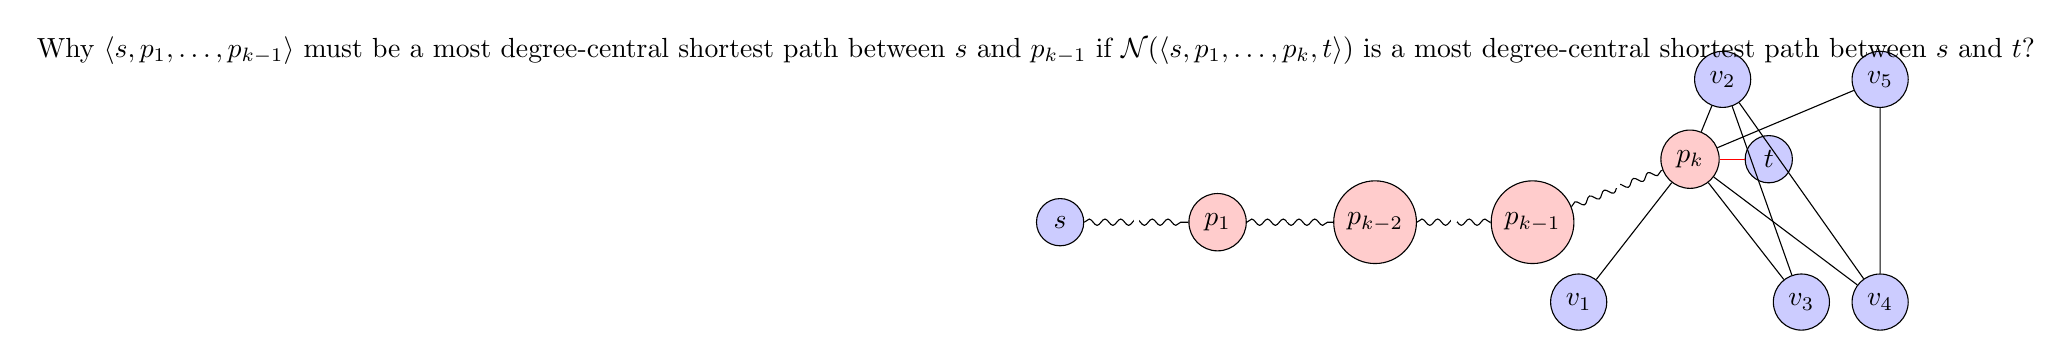
\begin{tikzpicture}[->, node distance = 2cm,
  block/.style = {circle, draw, fill=blue!20, minimum size=6mm},
  dot/.style = {circle, draw, fill=red!20, minimum size=6mm},
  label/.style = {fill=white, inner sep=1pt},
  curvedarrow/.style = {decoration={snake, amplitude=.4mm, segment length=2mm}, decorate}
]
\node[block]   (s)   {$s$};
\node[dot]    (p1) [right of=s]{$p_1$};
\node[dot]    (p2) [right of=p1]{$p_{k-2}$};
\node[dot]    (p3) [right of=p2]{$p_{k-1}$};
\node[dot]    (p4) [right of=p3, yshift=8mm]{$p_k$};
\node[block]   (t)   [right of=p4, xshift=-1cm]{$t$};

\path (s) edge [-, curvedarrow] node [pos=0.5, above, label] {} (p1)
      (p1) edge [-, curvedarrow] node [pos=0.5, above, label] {} (p2)
      (p2) edge [-, curvedarrow] node [pos=0.5, above, label] {} (p3)
      (p3) edge [-, curvedarrow] node [pos=0.5, above, label] {} (p4)
      (p4) edge [-, red] node [pos=0.5, above, label] {} (t);

\node[block]   (v2)  [above right of=p4, yshift=-4mm, xshift=-1cm]{$v_2$};
\node[block]   (v5)  [above right of=t, yshift=-4mm]{$v_5$};
\node[block]   (v1)  [below left of=p4, yshift=-4mm]{$v_1$};
\node[block]   (v3)  [below right of=p4, yshift=-4mm]{$v_3$};
\node[block]   (v4)  [below right of=p4, yshift=-4mm, xshift=1cm]{$v_4$};

\draw[-] (p4) -- (v2);
\draw[-] (p4) -- (v5);
\draw[-] (p4) -- (v1);
\draw[-] (p4) -- (v3);
\draw[-] (p4) -- (v4);

\draw[-] (v2) -- (v3);
\draw[-] (v2) -- (v4);
\draw[-] (v5) -- (v4);

\node at (current bounding box.north west) {Why $\langle s, p_1, \ldots, p_{k-1} \rangle$ must be a most degree-central shortest path between $s$ and $p_{k-1}$ if $\mathcal{N}(\langle s, p_1, \ldots, p_{k}, t\rangle)$ is a most degree-central shortest path between $s$ and $t$?};
\end{tikzpicture}
\end{document}